\documentclass[final,journal,letterpaper]{IEEEtran}
%\IEEEoverridecommandlockouts

%------------------------------------------------------------------------------

\usepackage{cite}
\usepackage{amsmath}
\usepackage{amsfonts}
\usepackage{amssymb}
\usepackage{graphicx}
\usepackage{url}
\usepackage{cite}
\usepackage{balance}
\usepackage{float}
\usepackage{threeparttable}

\usepackage{mathptmx}
\usepackage[scaled=.90]{helvet}
\usepackage{courier}

\usepackage{listings}
\usepackage{listings}
\lstset{
   language=C,
   basicstyle=\small,
   keywordstyle=\bfseries,
   identifierstyle=\ttfamily,
   stringstyle=\ttfamily,
   numbers=left,
   numberstyle=\tiny,
   stepnumber=1,
   numbersep=-5pt,
   showstringspaces=false
%   frame=single %trbl%
}

\usepackage[normalem]{ulem}

%------------------------------------------------------------------------------

\newcommand{\etal}{\emph{et al.}}
\newcommand{\eg}{\emph{e.g.}}
\newcommand{\ie}{\emph{i.e.}}
\newcommand{\etc}{\emph{etc.}}
\renewcommand{\baselinestretch}{0.97}\normalsize
%------------------------------------------------------------------------------

\begin{document}

%------------------------------------------------------------------------------

\title{A First Effort for a Distributed Segment-based Approach on Self-Assembled Nano Networks} 

\author{Vincenzo~Catania, Andrea Mineo, Salvatore Monteleone~and~Davide~Patti% 
\thanks{The authors are with the Dipartimento di Ingegneria
Elettrica, Elettronica ed Informatica, Universit\`a di Catania, Italy
(email: \{vincenzo.catania,amineo,salvatore.monteleone,davide.patti\}@dieei.unict.it).}}

\maketitle

%------------------------------------------------------------------------------

\begin{abstract}
In this paper we present DiSR, a first effort for a distributed
segment-based approach to routing and defect mapping in a nano-scale,
topology agnostic scenario based on DNA self-assembly. The main aim is
exploiting the already-proven qualities of segment-based routing
without neither requiring a topology graph as input, nor needing a
centralized algorithm to configure network paths.  After introducing
the conceptual elements and the execution model of DiSR, we show how
the opensource Nanoxim platform has been used to evaluate the proposed
approach in the process of discovering irregular network topology
while establishing network segments.  Results show how DiSR still
preserves some important properties (coverage, defect tolerance,
scalability)  while avoiding centralized tree-based broadcasting and
resource hungry solutions such as virtual channels and hardware
redundancy. Finally, we analyzed a first, not yet optimised gate-level
hardware implementation of the required control logic and storage for
DiSR, demonstrating a relatively acceptable impact ranging from 10 to
about 20\% of the budget of transistors available for each node.
\end{abstract}

%------------------------------------------------------------------------------
%\IEEEkeywords{...}

\begin{IEEEkeywords}
Nanotechnology, DNA, Self-assembly, Routing
\end{IEEEkeywords}
%------------------------------------------------------------------------------


\section{Introduction and Motivation}

Exploring long term alternatives to the CMOS technology is gaining
more and more relevance as the scaling trend of such devices keeps
introducing new challenges: power density, defect tolerance, testing
costs and wire delays are only a few of the many critical aspects
involved~\cite{itrs13}. 
While software parallelism and multicore
approaches~\cite{horowitz2004} and \cite{powell2009} are partially mitigating the impact of such
constraints on performances, it is likely that the growing computing demand will
eventually need even more radical architectural modifications and new
paradigms in order to address the Computer Design challenges of the next
decades.

In the last years, self-assembled nanoscale architectures~\cite{yan2003}
emerged as a promising technology due their tera/peta scale of
integration, defect tolerance and huge potential computing
capabilities. These technologies are certainly still at
their early stage of development, however different laboratory demos and
prof-of-concepts architectures have been presented~\cite{patwardhan2004, patwardhan2006_1, pistol2009}.
%, patwardhan2006
The main idea behind this approach is exploiting the physical regularity and
stability of DNA structures in order to create a scaffold onto which
nano-devices (e.g. nanowires and CNFETs~\cite{bachtold2001, tans1998, cui2001}) can be
attached. This can be achieved by designing appropriate complementary DNA tags for
each terminal to be placed, so that a nano device will be attached
only where its own DNA tag matches a complementary tag on the DNA grid
scaffold (see Figure~\ref{fig:nana}-a).
A detailed description of the chemical properties involved is far
beyond the scope of this paper (see also~\cite{braun1998, seeman1999}), so we will focus on
the three main challenges that this new fabrication process introduces
in Computer Design: \emph{(i) limited node complexity}, \emph{(ii) large scale
randomness} and \emph{(iii) high defect rates}.  

The \emph{limited node complexity} aspect is directly
related to the use of complementary DNA tags in order to place circuit
components. In a traditional CMOS process the complexity is introduced
using a photolithography mask, so that larger (more complex) circuits
only require larger masks; conversely, self-assembly achieves
complexity by increasing the number of unique DNA tags, since more
different tags means having more control on component placement. Ideally, by specifying a single
and unique tag for each nano transistor terminal, we could exactly
choose where each component would be placed. But the number of DNA
symbols forming the DNA sequence is limited (sequence of 4 nucleobases
G,A,T,C) and so creating many different tags (of a given length) would
mean make them more similar to each other, increasing the probability
of incorrect/partial matching. To avoid this problem we should limit
the number of unique tags, thus limiting the complexity at each node.
In particular, a budget of about $10,000$ CNFETs per node has been
estimated in~\cite{liu_jetcs}.

\emph{Large scale randomness} is the other fundamental condition of
self-assembled technology: DNA tags allow a control placement inside
node grid, but there is no control of where each of these  grids will
be placed on the whole network. As a consequence, other typical
properties of regular networks cannot be guaranteed, e.g. being
connected to a fixed number of neighbors, having a determined
orientation and so on.

Finally, \emph{defect rates}: while they are very hardly tolerated in mask
based top down design, the same nature of a bottom up self-assembly
 process cannot assume such a deterministic device placement
process, thus defect tolerance is something like a design requirement
more than an exception to be avoided.

\begin{figure*}
\centering
\begin{tabular}{cc}
    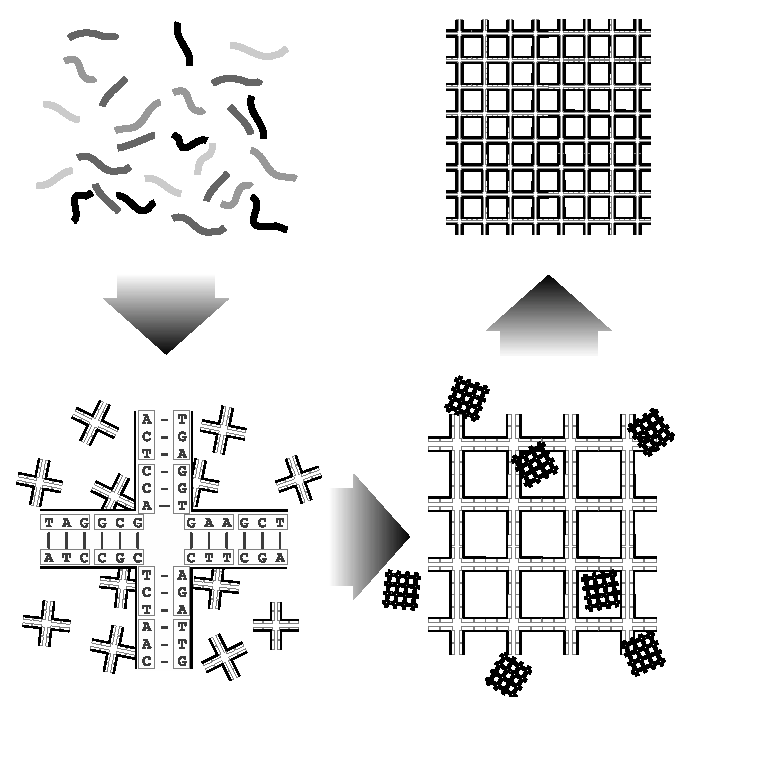
\includegraphics[width=0.40\textwidth]{pictures/dna2b.eps} &
    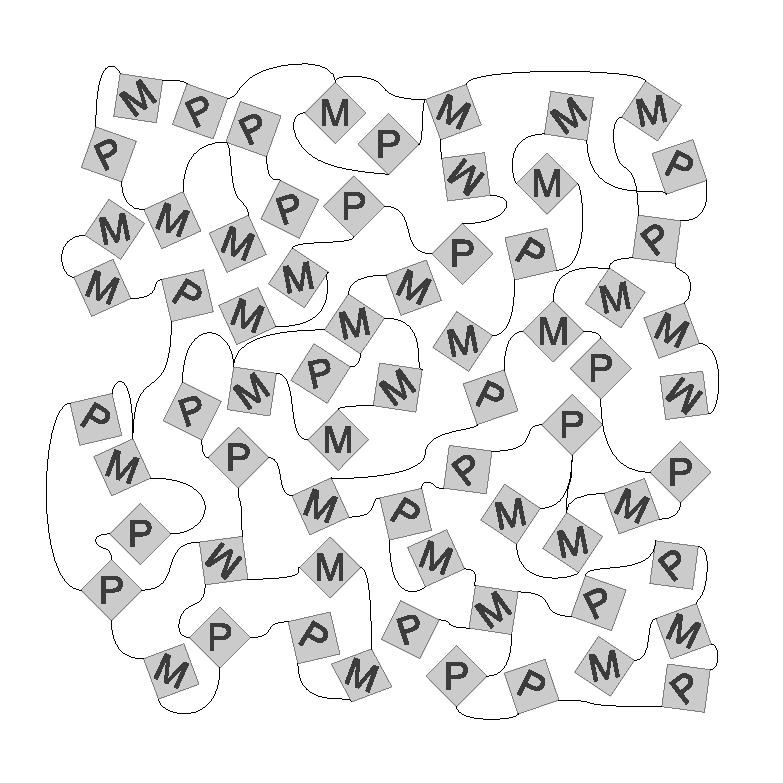
\includegraphics[width=0.40\textwidth]{pictures/dna1_complex2.eps} \\
 (a) & (b)
 \end{tabular}
  \caption{(a) DNA tag matching and (b) resulting irregular topology}
  \label{fig:nana}
\end{figure*}
These aspects of a DNA self-assembly process lead to some important
implications to be addressed when approaching to the design of
a computer architecture: computational model should be based on a
distributed network of small processing and storage nodes, randomly
placed and interconnected (see Figure~\ref{fig:nana}-b).
Proof-of-concept of such architectures can be found for
example in~\cite{patwardhan2006_1}, where instruction and data
operands are move around the network in order to be processed.
Independently from the particular policy chosen for routing packets,
such networks must be able to guarantee deadlock freedom without any
prior assumption on topology.

In this work we introduce \disr{}, a Distributed Segment-based approach
to deadlock freedom in large scale DNA self assembled networks. Our
contribution aims to achieve the classical properties of a
segment-based approach~\cite{mejia_ipdps06} without requiring any
topology graph, external defect map or centralized algorithm
execution.  So the \disr{} approach is not intended to discover the
``optimal'' segment choice (ideally reachable with the knowledge of
the topology graph) but just to demonstrate a concrete model that can
fit into such complex, irregular and large sized networks.
It is important to
underline that, although we can assume an architecture similar to the
one depicted in Figure~\ref{fig:nana} as background, the topology discovery
problem faced in this work is more general and not strictly dependent on any of the
underlying computing architecture.

The paper is organized as follows: in Section~\ref{sec:related_works}
we summarize the main approaches to topology agnostic routing. Next in
Section~\ref{sec:disr_concepts} are described the main elements and
the execution model of the proposed approach.  In Section~\ref{sec:simulation}
simulations are carried out with the open-source tool Nanoxim to
demonstrate how \disr{} preserves some of the main segment-based
properties and how compares to the tree-based approaches. Finally a
draft of a architectural implementation is shown in
Section~\ref{sec:implementation} to evaluate the feasibility of the
approach in terms of node complexity.

\section{Background and Contribution}
\label{sec:related_works}
Several works addressed the problem of topology agnostic deadlock
freedom introducing virtual channels~\cite{sancho2002, skeie2002,
skeie2004, koibuchi2003}, but while they show interesting
performances, the low resources deadlock makes them not suitable for
the specific DNA self assembled networks we are assuming as
background.
Other topology independent algorithms~\cite{schroeder1991,
koibuchi2001, cherkasova1996} do not require any virtual channels but
exploit the concept of ``turn prohibition''.
In particular, authors of~\cite{Patwardhan05evaluatingthe} exploits the creation of a spanning tree of the
topology, placing bidirectional restrictions by avoiding a packet
to traverse the same link in both up and down directions.
The hierarchical nature of this approach can lead to uneven traffic
distribution, with many packets traversing upper links (near to the
root), but this is quite acceptable in classical wide area networks
topologies with a limited number of nodes. Other approaches such as
FX~\cite{sancho2000} mitigate this
issue, but the set of turn restrictions is still prefixed,
strictly depending on the particular tree root selected. 
Other solutions try to approach the issue of irregular
topologies by limiting the number~\cite{duato1997, gomez2004, koibuchi2008} or the
location~\cite{zhang2008, flich2008, liu2011} of missing links. This
restriction is clearly unacceptable given the hight-defect rates of
DNA self-assembled networks scenario. For the same reason, we also
avoid considering solutions based on hardware-redundancy to
dynamically recover defects as in~\cite{constantinides2006, kohler2010,  park2006, ebrahimi2013}. 

In~\cite{mejia_ipdps06} authors present an approach the solves these
limitations by allowing turn restrictions to be placed locally,
independently from other restrictions. The whole network is
partitioned into segments, and a bidirectional turn
restriction can be freely chosen within a segment in order to guarantee
deadlock freedom while preserving network connectivity. This \emph{locality
independence} property, avoiding the requirement of any particular tree/root
choice, would make it the best choice for the given scenario;
however, it still requires the knowledge of the
whole network graph in order to find the segments. 

The \disr{} approach presented in this work is a first attempt of
achieving the same goals of a segment based turn prohibition  without
requiring any topology graph or centralized execution. In particular
\disr{} implements segment discovery and turn prohibition using a
completely different mechanism, based on a distributed exchange of
small setup packets requiring on average $15\%$ of the available
resource budget. The following main features distinguish \disr{}
from classic approaches to segment partitioning: 
\begin{itemize}
\item No centralized entity is globally responsible and/or aware of
what is going on, i.e. the status of the \disr{} execution is
collectively distributed among the nodes
\item  No defect map and/or topology graph is used as input,
thus, the topology has to be discovered \emph{while} segments are
created
\item At the end of the execution, no segment list is created or
stored anywhere: each node is only aware of belonging to some segment,
ignoring the presence of other nodes in the same segment and even the
presence of other segments in the network
\end{itemize}




%------------------------------------------------------------------------------
\section{Preliminary concepts}
%------------------------------------------------------------------------------
\label{sec:disr_concepts}

\subsection{Basic Idea}
The main concept behind of the original SR approach is the
\emph{Segment}: a Segment is basically a path of consecutive node
and links. All segments start with a link attached to a node which
belongs to different segment, ending with a link also attached to a
node belonging to a different segment. A exception is the first
segment estabilished in the network, called \emph{starting segment} which is  a loop
beginning/ending on a particular node defined as bootstrap node.

The idea is to partition the network in a set of disjoint segments, and then
placing a turn restriction within each segment. It has been proved~\cite{mejia_ipdps06}
that such a set of turn prohibitions guarantees dealock freedom and
while preserving connectivity of the network.

Describing the execution phases of DiSR from a top level point-of-view
is basically similar to the classic SR approach. This can be useful to
give an initial idea of the approach, however, some essential
differences should be pointed out. First of all no centralized entity is
globally aware of what is going on: the status of the DiSR execution
is collectively distributed among the nodes; second, no defect map and/or
topology graph is available as input, thus, the topology has to be
discovered \emph{while} segments are created; finally, at the end of the
execution, no segment list is created: Each node is only aware of
belonging to some segment, ignoring the presence of other nodes
in the same segment and even the presence of other segments in the
network.

Roughly speaking, the execution of can be described as the execution
of the following phases:
\begin{itemize}
\item Injection of the DiSR process from upper layer to set a bootstrap
node
\item Bootstrap node broadcasting to create the first segment of the subnet
\item Parallel requests starting from assigned node to discover other segments
%\item Turn proibition in each confirmed segment
%\item Draining of remaining packet due timeouts
\end{itemize}

Once again, it should be pointed out that nowhere in the network there
is such a global vision of these exection phases. A more detailed
description of the exection model at each node is discussed in the
next section.

\subsection{Packets types Required}

The DiSR approach works with a distributed mechanism which is build
upon an exchange of small packets containing the following fields:
\begin{itemize}
\item{packet\_type}: encodes the meaning of the control message respect
to the whole DiSR process.
\item{seg\_ID}: the id of the segment associated to the DiSR control message
\item{src\_id}: the id of the node that initially originated the
packet
\end{itemize}

As regards packet\_type, we can have the following control packets:
\begin{itemize}
\item{\texttt{STARTING\_SEGMENT\_REQUEST}}: Injected by the bootstrap
node to when searching for the first segment. 
\item{\texttt{STARTING\_SEGMENT\_CONFIRM}}: used when estabilishing
the starting  segment. 
\item{\texttt{SEGMENT\_REQUEST}}: used to search candidates for a segment (not the
first)
\item{\texttt{SEGMENT\_CONFIRM}}: used to estabilish a segment. 
\item{\texttt{SEGMENT\_CANCEL}}: used to cancel the process of searching a segment along a
specific link.
\end{itemize}

A quantitative analysis of the resources needed to implement these
fields is presented in Section~\ref{sec:implementation} when
discussing the impact of the DiSR control logic and storage on
hardware implementation of the node.

\subsection{DiSR Data Structures}
\label{ssec:disr_dstruct}

We distinct between two different kind of data stored at each node:
\emph{Local Environment Data} (\emph{LED}) and \emph{Dynamic Behaviour
Status} (\emph{DBS}).

The \emph{LED} is like a snapshot of the DiSR algorithm at each node,
consisting in the following variables:

\begin{itemize}
\item{\emph{segID}}:a value used to specify the segment to which the
node has been assigned or is candidate for being assigned.
\item{\emph{visited}}: a boolean value. When \emph{true}
a \emph{segID} different from \texttt{NULL} specifies the segment 
to which the node has been assigned. 

% TODO: the following is true, but complicates things at this stage
%Note that a value different from \emph{NULL} does not
%necessarily mean the node has been assigned to some segment (e.g. when
%searching starting segment is set \emph{visited} by default even if not yet
%assigned to any segment). 

\item{\emph{tvisited}}: a boolean value. If \emph{true}, the node is
being considered as candidate for a segment, and the \emph{segID} value
specifies the segment id for which the node is candidate. 
\item{\emph{link\_visited[]}}: an array
of values representing information about attached links, that is, the
segID of the segment owning each link. When \texttt{NULL}, the corresponding link has not yet been
assigned.
%TDB: do we need to introduce some value for the
%“bridge” status ? (e.g. a node connecting the terminal node of a
%subnet with the starting one of another) 
\item{\emph{link\_tvisited[]}}: an array of
values representing information about attached links, that is, the \emph{segID} of
the segment for which the link is candidate. When \texttt{NULL}, the link is
currently not \emph{tvisited}.  
\end{itemize}
%\item{\emph{starting}}: boolean, \emph{true} if the node is a
%starting node from which the whole process was initiated.
%\end{itemize}

In addition to the \emph{LED} variables described above, further
information should be stored in order to capture the current dynamic
behaviour of the node. This is represented by \emph{DBS} variable,
which strictly depends on the \emph{LED} data and the events occurring
at the node. The \emph{DBS} can have the following values:

\begin{itemize}
\item{\emph{Free}}: a node that has  not been yet considered  by the DiSR algorithm.
The node is not marked as \emph{visited}/\emph{tvisited}.
\item{\emph{Bootstrap}}: a node which has been explicitly set as bootstrap node from
an upper layer via. 
% TODO: this and all the other details on the items below should be
% checked and moved elsewhere for a future long paper

%This is required because a
%\texttt{STARTING\_SEGMENT\_REQUEST} packet should be injected in order to start
%the whole process.
\item{\emph{ActiveSearching}}: a node from which a find process of new segments has
been started and not yet cancelled or confirmed. 
%This happens when all
%the following conditions are matched: the node is marked as \emph{visited},
%that is \emph{visited} = TRUE 
%TODO: \emph{segID} is set to some value reflecting
%the segment request sent there is a link that is being investigated by
%the node, that is a tvisited\_link marked with the same id of the node 
\item{\emph{Candidate}}: a node currently candidate for belonging to some segment
with id segid, not being itself the node from which the find process
was started. 

%The following conditions should be matched: \emph{tvisited} =
%true, with segID=X different from node's id.  Two links set as
%\emph{link\_tvisited} with id X. Let’s refer them as  links 'i' and 'j'. Then
%link\_tvisited[i] was set = X when the find process from an adjacent
%node reached the current node, while link\_tvisited[j] has been set to
%X when the node itself started to investigate its free links for the
%segment request with id X. Note that while investigating its attached
%links, if the find process fails along path 'j', the current node can
%investigate another free node 'k' if suitable.  
\item{\emph{CandidateStarting}}: same as above, but the node is currently being considered as candidate
for starting segment. 

%Two main differences: Can confirm
%\texttt{STARTING\_SEGMENT\_CONFIRM} with the same \emph{segID} when receiving a normal
%\texttt{SEGMENT\_REQUEST}: Overwrites its status setting it to \emph{Candidate} for the
%segID frees the links previously set as \emph{tvisited} during flooding
\item{\emph{Assigned}}: a node for which the segment has been determined.  The
segment \emph{segID} attribute value is set to some id X different from \texttt{NULL}.
%The \emph{visited} value is \emph{true} NOTE: an \emph{Assigned} state is a quick temporary
%state, since it becomes \emph{ActiveSearching} if a not (\emph{visited}/tvisited)
%link is suitable for searching new segments (see next\_visited
%procedure on paper) 
\end{itemize}


\subsection{Sketch of DiSR}

\begin{itemize}

\item{\textbf{Injecting bootstrap request}}: all nodes have a initial
\emph{DBS} status \emph{Free}, except for a
 node with status \emph{Bootstrap}, set by some signal from an
upper layer via. When starting, this bootstrap node sets itself as \emph{visited} and
changes its status to \emph{ActiveSearching}, injecting a
\texttt{STARTING\_SEGMENT\_REQUEST} across one of its free links. 

\item{\textbf{Flooding}}: Each node receiving a \texttt{STARTING\_SEGMENT\_REQUEST},
if not yet (\emph{visited}/\emph{tvisited}),  forwards it to its free links using a flooding mechanism.
Each of these links is then marked as \emph{tvisited} with the segment id
associated to the request. Note that a node that has already received a
\texttt{STARTING\_SEGMENT\_REQUEST} packet can simply ignore further packets
associated to the same request, having already contributed to the
flooding. 
%Note also that each of these packets has a max\_segment\_hops
%field to prevent packets from travelling undefinitively.  

\item{\textbf{Confirming the Starting Segment}}: when this \texttt{STARTING\_SEGMENT\_REQUEST} packet reaches
the starting node (from a different link, of course), the starting
segment is found. Then the starting node sends back a \texttt{STARTING\_SEGMENT\_CONFIRM}
packet with the same id along the link from which it received the
\texttt{STARTING\_SEGMENT\_REQUEST}. Each node do same by changing its own status
to \emph{Assigned}. So the confirmation packet is sent back from
node to node and the starting segment is created. 

Note: A node knows to be \emph{Candidate} due a
\texttt{STARTING\_SEGMENT\_REQUEST}.  Then, when receiving a simple
(not starting) \texttt{SEGMENT\_REQUEST} , it can simply cancel its
previous \emph{Candidate} status, since this second
request means that the starting segment has already been found. 

%What happens to nodes not receiving these segment request?
%they simply remain \emph{tvisited} and after a timeout reset their
%state as free. But they could also remain \emph{tvisited} for the
%starting segment, since this doesn’t affect their behaviour for future
%segment requests.  

%failure: TODO should we handle this case ? i.e.  marking as terminal ?

\item{\textbf{Injecting other request}}: Each node in the \emph{Assigned} status can initiate a search for a
segment, by sending a \texttt{SEGMENT\_REQUEST} across one of its free
links. Note that, since this is not the starting segment, in this case
the packet should not return back to the initiator, but just another visited
node
\item{\textbf{Setup of a segment}}: The find process is successfull
when an \emph{Assigned} node receives the \texttt{SEGMENT\_REQUEST} packet. Then, a \texttt{SEGMENT\_CONFIRM} is
sent back along the path that originated the request.  
\item{\textbf{Failing while searching a segment}}: a node received a \texttt{SEGMENT\_REQUEST} packet but
matched one of the following conditions: the node is free but has no
more suitable free links (can’t forward the \texttt{SEGMENT\_REQUEST}) the node
is \emph{tvisited} candidate for another find process the request packet
exceeded the max\_segment\_hops limit.  In all these cases the node
sends back a \texttt{SEGMENT\_CANCEL} along the proper link modifying its state
to free. Each of the subsequent nodes will forward this \texttt{SEGMENT\_CANCEL}
only if no more free links can be explored starting from them.
\end{itemize}


%\subsection{Intra-node vs Inter-node parallelism}
%In the processes described above, we assumed that each node in the
%READY\_SEARCHING state can start a find segment process by injecting a
%\texttt{SEGMENT\_REQUEST}. However, a more accurate decision when defining DiSR
%should be made in order to decide whether or not the node must
%actually perform this action. 
%The point above is is strictly related to the general question: which
%level of “parallelism” should we allow in DiSR ? The adopted approach
%is that, although the nature of DiSR itself is intrinsicly parallel,
%the use of parallelism makes things work in a more complex way. In
%other words, DiSR is parallel when needed, but it does not exploit
%parallelism as an “improving feature”. When not needed, things should
%be serialized. For example: when a node is “ready searching” could
%start several find segment process associated to the same segment, one
%for each free link. But serializing this by investigating the free
%links in order could be a simplest solution. We refer to this saying
%that we avoid intra-node parallelism.  Note that while intra-node
%parallelism can be avoided, trying to avoid inter-node parallelism
%could be more complex than allowing the parallelism itself. Imagine
%for example the effort of trying to coordinate nodes so that an unique
%finding node process is actually running in the whole subnet. Thus, in
%contrast to the intra-node parallelism, the inter-node parallelism is
%a structural property of the DiSR algorithm and should not be avoided.
%------------------------------------------------------------------------------

\section{Detailed Node behaviour Model}
\label{sec:disr_detailed_model}

The \emph{LED} variables at each node are are initially set so the node and
each of its links is set as free. The only node that makes exception
is the bootstrap node, initialized in the \emph{Bootstrap} status. All
the subsequent events happening at each node are the consequence of
its current dynamic status (DBS) and the packets received.

%TODO: add state machines

% TODO: fix, move elsewhere or delete
%Assumption: when discussing of visited/\emph{tvisited} nodes, we are assuming
%with an id corresponding to the same subnet. Nodes involved in other
%subnet processes can simply ignore these packets. (TBD: formalize more
%clearly in which cases inter-subnet packets must be ignored, probably
%this happens most of the times, but in some cases, e.g. when a
%terminal node is found, some kind of communication packets are needed
%in order to crearte the bridge between two subnets.) 

\subsection{Receiving a \texttt{STARTING\_SEGMENT\_REQUEST}}

The request for the first segment should be managed differently since
all nodes (except the starting one) must forward the packet using a
flooding mechanism. This is necessary since the request packet must
return the bootstrap node.
When a node receives a \texttt{STARTING\_SEGMENT\_REQUEST}, the
following cases can happen:

\begin{itemize}
\item The node is not candidate or assigned: it should set itself as
\emph{Candidate} and forward the packet along its free links, using
flooding.  
\item The node is \emph{Candidate} with the same
\emph{segID} and \emph{src\_id} is equal to node id: this means the
node was the initiator of the request, so a starting segment was found and
should be confirmed sending back a \texttt{STARTING\_SEGMENT\_CONFIRM}
packet.  
\item The node is \emph{Candidate}, with the same \emph{segID} of the
packet but \emph{src\_id} is different from node id: due
the flooding mechanism, another starting segment packet reached a node
which was previously marked as \emph{Candidate} from the same starting segment
search process. Since the node is candidate with the same id, it means
that it already accomplished in the task of propagating that kind
packets, thus can simply ignore the event thrashing the packet.  
%TBD: how the status should be changed ? depend on the flooding mechanism. Note
%that these links do not include the link from which the request was
%received.  
\item The node is \emph{Candidate}, with a different \emph{segID}: 
this simply means that the starting segment received is deprecated,
because the node has already accepted non-starting segment requests
originated from other \emph{Assigned} nodes.
\item The node is \emph{Assigned}, with a different \emph{segID}:
same as the previous case. 

% TODO: check and remove, the below is not true
%CHECK:  it is not the initiator of the starting segment request, but
%is already assigned to some segment!? assuming again we are discussing
%of nodes belonging to the same subnet, this should NOT happen, since
%the only visited node of the subnet should be the initial node from
%which the \texttt{STARTING\_SEGMENT\_REQUEST} originated. Note again that we are
%assuming that if the the node is visited or \emph{tvisited} with the id of
%another subnet can simply ignore the request.  The node is \emph{tvisited}
%but it is not the initiator of the request (different id): same as
%above, if we are assuming nodes of the same subnet, this should not
%happen. If the node is of another subnet, can simply ignore the event.

\end{itemize}

\subsection{Receiving a \texttt{SEGMENT\_REQUEST}}
When a node receives a \texttt{SEGMENT\_REQUEST}, the are the following cases:

\begin{itemize}
\item The node is \emph{Assigned}: a segment was
found and it should be confirmed sending back a \texttt{SEGMENT\_CONFIRM}
packet.  
\item The node is \emph{Candidate}: it should discard the packet sending
back a \texttt{SEGMENT\_CANCEL} 
\item The node is not \emph{Assigned} or \emph{Candidate} and has free
links: it marks itself as \emph{Candidate} and forwards the \texttt{SEGMENT\_REQUEST}
to one of its free links, according to some internal ordering
\end{itemize}

NOTE: the main difference between confirming a \texttt{STARTING\_SEGMENT\_REQUEST}
and confirming a \texttt{SEGMENT\_REQUEST} is that in the first case the node
itself is included in the segment , while in the second case the
receiving node does not belong to the segment found. 

%The motivation is
%that in the second case the node was already marked as \emph{visited} because
%of being assigned to some segment found before, while in the
%starting-segment case, by definition, the first segment of a subnet
%begins with the starting node, which is marked as \emph{visited} by the SR
%algorithm when searching for the first (starting) segment. Remember
%that the first segment of a subnet is a loop beginning with the
%starting node. 

\subsection{Receiving a \texttt{SEGMENT\_CONFIRM}}
When received, if the node status is \emph{Candidate} with a \emph{segID} corresponding to the one indicated in
the packet, the node learns to belong to the segment associated to the
id. Further, it should forward this packet to the link where the
original \texttt{SEGMENT\_REQUEST} packet came from, so that all candidate nodes
can learn the segment id they belong to.  \emph{LED} shoud be
updated: The state of the node changes from \emph{tvisited} to \emph{visited}.  the
\emph{link\_tvisited} previously set with the \emph{segID} should be invalidated the
\emph{link\_visited} variable associated to the incoming confirm should be set
as segID. Note that if the request was flooded across different links,
the \emph{link\_visited} variable associated to the other paths should not be
set.  the \emph{link\_visited} variable associated to the link from which the
request was originated should be set segID

\subsection{Receiving a \texttt{SEGMENT\_CANCEL}}
When a node receives a \texttt{SEGMENT\_CANCEL} packet it means that searching
for a segment along that path was unsuccessful. But if the node still
has other free links to try, it should forward a \texttt{SEGMENT\_REQUEST} to
the next link (next according to some internal ordering). So a node
forwards back the \texttt{SEGMENT\_CANCEL} packet along the link that originated
the \texttt{SEGMENT\_REQUEST} packet only when there are no more free links to
try. If this is the case, the node modifies its status from
\emph{Candidate} to \emph{Free} and forwards the \texttt{SEGMENT\_CANCEL} packet to the link from which
the request was received. The process stops when the \texttt{SEGMENT\_CANCEL}
packet reach the starting node that originated the request.

%TODO REPEAT!!
%When a node discovers that the path that includes
%the node itself is no more suitable, a \texttt{SEGMENT\_CANCEL} is sent back
%across the link from which the \texttt{SEGMENT\_REQUEST} was received.  Possible
%reasons for that: The node it’s already candidate for another segment
%The node it’s free but can’t find a free link (according the
%cyclelinks timeout) The node it’s \emph{tvisited} for the same request id,
%previously forwarded that request along some free direction, but now
%it’s receiving a a cancel request and has no more free links


\section{Simulation and Results}
\label{sec:simulation}

In this section we will test the proposed \disr{} approach to demonstrate
its effectiveness and compare it against topology agnostic approach
based on spanning trees and
broadcasting~\cite{Patwardhan05evaluatingthe}, to measure how \disr{}
performs in covering the network structure.

%\item Against the centralized segment based approach (SR), to evaluate
%if and how its known properties are still preserved in the new nano-scale distributed scenario

\subsection{Nanoxim Environment}

In order to quantitatively and qualitatively evaluate the proposed approach a
specific simulation environment has been developed, resulting in
the open source and freely available project called
Nanoxim~\cite{nanoxim}.
Nanoxim is a SystemC tool based on a almost rewritten
version of the Noxim Network-on-Chip simulator~\cite{noxim}. While some
complex features have been removed (e.g. wormhole, congestion/topology
aware routing and selection strategies) new features specifically
taylored for the nanoscale scenario were introduced, e.g. the ability to simulate a random
network, the implementation of the \disr{} to obtain the segment topology
and the support for defective links and nodes.

%------------------------------------------------------------------------------
\subsection{Experimental setup}
The following parameters have been taken into account when
performing the \disr{} simulation:
\begin{itemize}
\item {\emph{Size of the network}}: number of nodes, on a range from
10x10 to 100x100 sized networks. 
%\item {\% defective links}: the probability that each link is
%disconnected or not present, from 0 the amount that yelds
%no more segments.
\item {\emph{\% defective nodes}}: the probability that a node is not
working, thus having all its links cannot be utilized during \disr{} setup.  
%Same range as defective links parameter.
\item {\emph{Bootstrap node}}: the node used from upper layer 
to inject the \disr{} process. When not explicitly investigating the
impact of each single bootstrap choice, a set representative regions have been
considered, e.g. the central part of the network and the edge corners.
\end{itemize}
To present the results, the following evaluation metrics have been adopted:
\begin{itemize}
\item{Node coverage}: this is the fraction of nodes that
are assigned to a segment. In the ideal case, all the non defective
nodes should be assigned, so this metric is useful to show how some
disconnected regions can negatively impact on the whole \disr{}
effectiveness.
\item{\emph{Latency}}: this measures how the cycles required to complete the
segment assignment scales for increasing network sizes and defect rates
\item{\emph{Bootstrap node effect}}: this evaluates the impact of the chosen
bootstrap node on the node coverage.
\end{itemize}

%Further, to evaluate how \disr{} compares against the centralized segment
%based algorithm, the following metrics have been adopted:
%\begin{itemize}
%%\item {Average Path Lenght}:
%%\item {Average Link Weight}:
%\item {Unidirectional restrictions:}
%\item {Number of Segments}:
%\end{itemize}

Since the distribution of defects and thus the resulting topology is randomly
generated, a set of simulations with different seeds has been run
for each system configuration. We found that 20 repetitions are
required in order to obtain statistically significant results.


\subsection{Results}
\label{sec:results}

In this section we analyze the results in terms of node
coverage and latency at different network sizes, defect rates and
bootstrap injection points.  In particular
Figure~\ref{fig:results_coverage} shows
node coverage for \disr{} and RPF tree based approach respectively. While
the first aim of \disr{} is not to reach the optimal coverage, we still
can observe a quite good performance as compared to the tree based
approach. Note that defect rates beyond 25\% lead to many disconnected
regions of nodes that \disr{} currently cannot handle.
For example Figure~\ref{fig:net} show a 30x30 network with a 25\%
defect in which the bottom-left part cannot be reached due
disconnected regions. Note that remaining defective nodes belonging to
connected regions are successfully surrounded by \disr{} coverage; in any
case, these defect levels should be considered as worst case scenarios, so the
achieved coverage of $0.5$ is a satisfying result for this first
version of \disr{}. On the other hand, the network size seems to have a
limited impact when defect rate do not introduce too much disconnected
regions. 
\begin{figure*}
\centering
\begin{tabular}{cc}
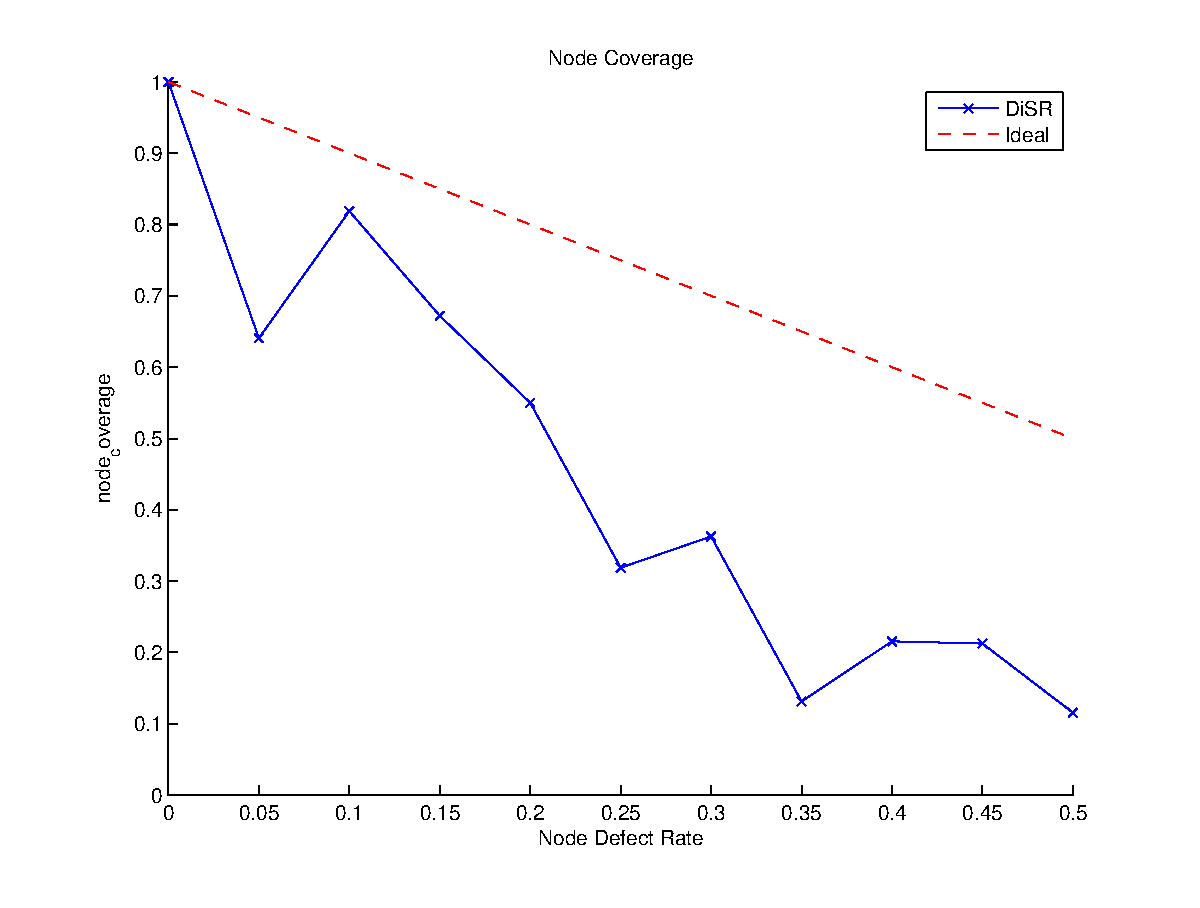
\includegraphics[width=0.48\textwidth]{pictures/set1.eps} & 
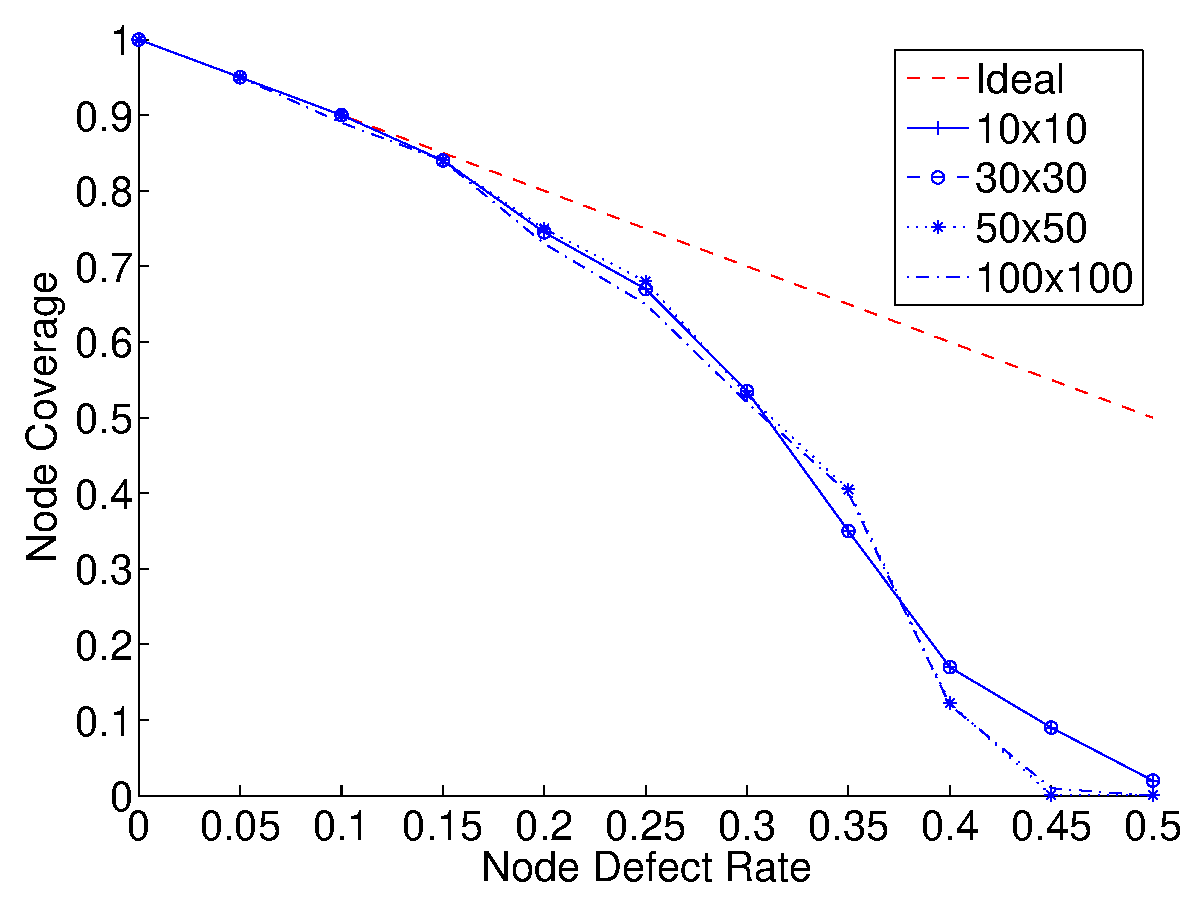
\includegraphics[width=0.48\textwidth]{pictures/coverage.eps} \\
(a) & (b) 
\end{tabular}
\caption{\disr{} (a) and RPF (b) node coverage}
\label{fig:results_coverage}
\end{figure*}

\begin{figure*}
\centering
\includegraphics[width=0.70\textwidth]{pictures/net.ps}
\caption{Covered regions in a 30x30 network with 25\% defects}
\label{fig:net}
\end{figure*}

\begin{figure*}
\centering
\begin{tabular}{cc}
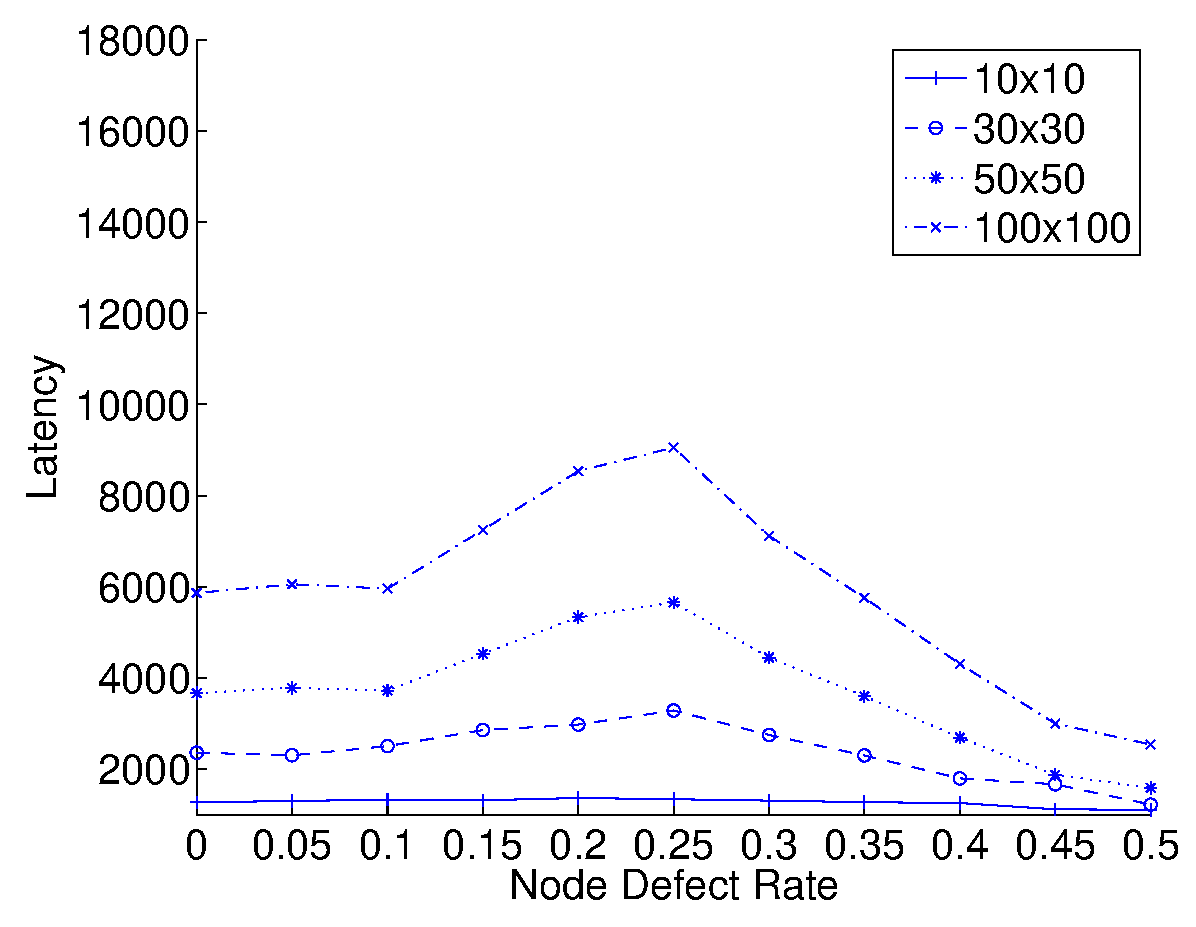
\includegraphics[width=0.48\textwidth]{pictures/set2.eps} & 
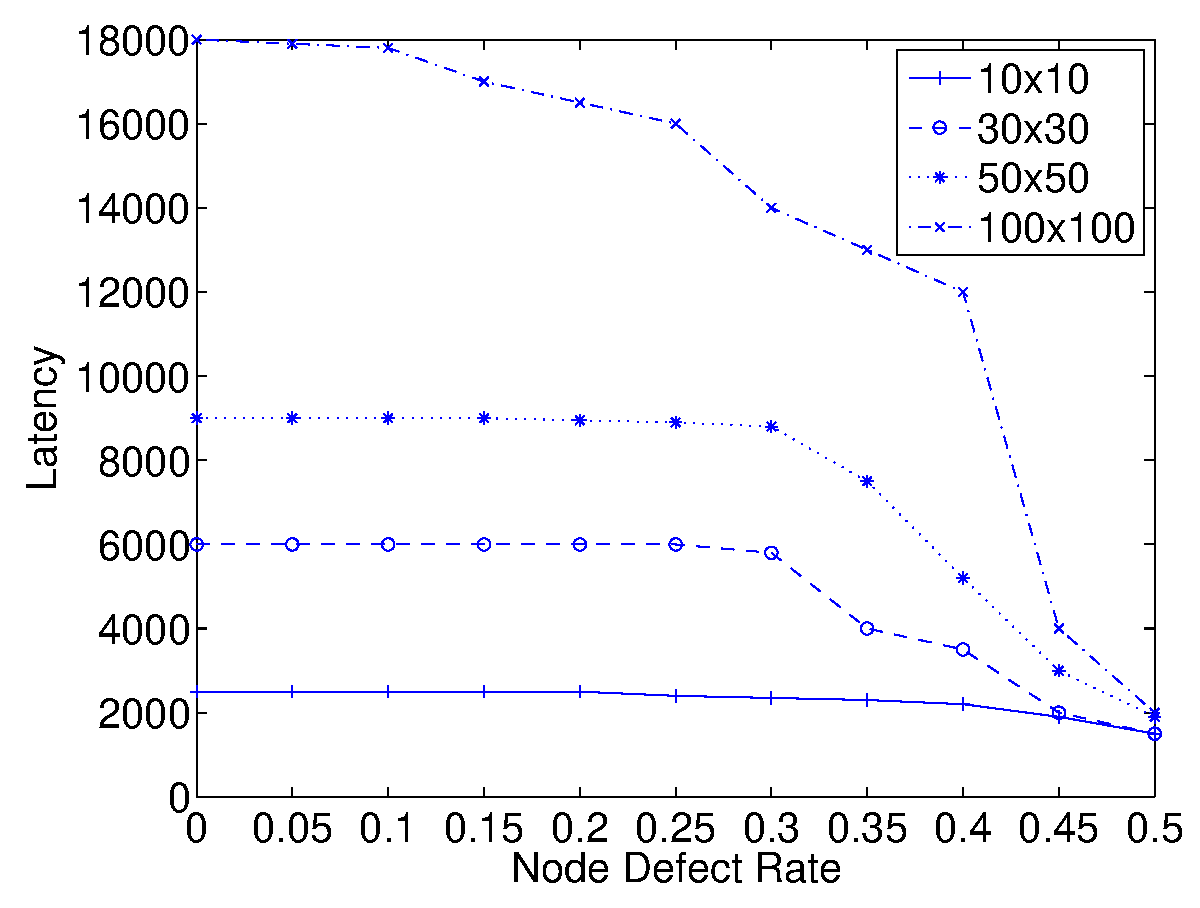
\includegraphics[width=0.48\textwidth]{pictures/set2_rpf.eps} \\
(a) & (b)
\end{tabular}
\caption{Latency of \disr{} (a) vs tree based RPF (b) }
\label{fig:results_latency}
\end{figure*}

The number of cycles required to complete segment mapping process
is shown in Figure~\ref{fig:results_latency}. In this case comparison
against tree-based shows better (lower) values at different defect
rates.  Rather than the absolute numbers, what it's more interesting
to observe is how \disr{} latency scales with network size. For example,
going from 900 to 2500 nodes, at the medium defect rate of $0.15$,
leads to an increase from 3000 to 4500 cycles. It should be noticed
also how the effect of defect rate is increasing until the threshold
of $0.25$ is reached, meaning that until that limit \disr{} finds it more
and more difficult to complete the process due increasing defective
paths, but still discover new segments when let running for a more
extended amount of cycles. This behavior is not reported in the RPF
based approach, meaning that a tree based approach, although starting
from higher values, is less affected by defect rates (when low rates
are considered).
After the $0.25$ threshold, the impact of entire disconnected regions
becomes predominant and both approaches become faster in completing
the covering process, since far less nodes can be actually reached. 

Finally, Figure~\ref{fig:results_bootstrap} visually represents  the
stability of the approach against choices of a different bootstrap
node in a 10x10 network.  This is an important aspect to evaluate when
considering that one of the main advantages of \disr{} against all the
tree based approaches should be the ability of choosing whatever
bootstrap node, without having to care about the role assumed in the
future by the chosen root node.  In other words, after segments have
been established, the bootstrap node is like every other node, i.e. it
is not center of a structure, and it is not an hotspot for the traffic
distribution. The results in terms of coverage,  shown for low, medium
and high defect profiles, demonstrate a relatively limited
impact of the bootstrap choice in the low/medium scenarios, while a
$30\%$ instability is found for very high defect rates. This also
sounds acceptable, since when a lot of defective nodes are present, the
particular position of the bootstrap node could lead to a completely
different evolution in the \disr{} setup process.

\begin{figure}
\centering
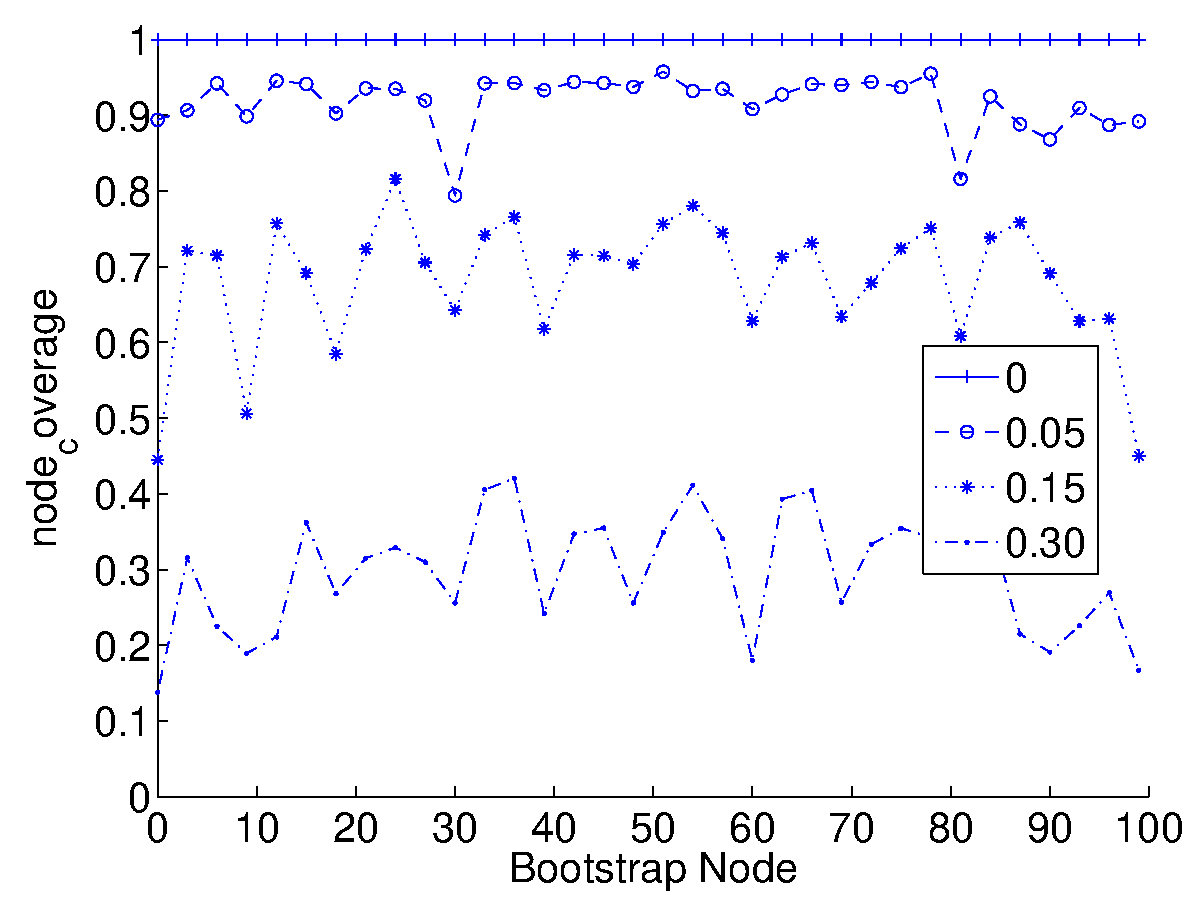
\includegraphics[width=0.48\textwidth]{pictures/set3.eps}
\caption{Effect of bootstrap node}
\label{fig:results_bootstrap}
\end{figure}

% TODO: long paper
\subsection{Other Optimisations}
Some optimisation parameters, which demostrated to improve the \disr{}
results have been fixed to some good values, but are not subject to
further investigation; once again the focus here is not the
optimal set of segments, but just demostrating a working approach. 
These are optimisations are:
\begin{itemize}
\item \emph{cycle\_links}: max number of retries across the set of links of
each node. While searching for a free link due an incoming request,
the same request is cancelled after a given number of tries. This
gives to preceding node change to test a different paths. Default is set to 1.
\item \emph{bootstrap\_timeout}: number of time units that a bootstrap node
should wait before assuming that a livelock in the starting segment
process has occurred. In the worst case, we can imagine that longest
path required is the one returning to the bootstrap node after having
travelled across all the links. So, althought this is just an extreme
situation, a good upper limit can be safely be set to NxN.
\item \emph{bootstrap\_immunity}: in order to avoid the failure of the whole \disr{}
setup process, a bootstrap node should not have defective links.
Enabling this optimisation, a bootstrap node is immune to defects.
We may think of a pre-bootstrap phase that properly selects (from upper
layer via) a bootstrap node which is tested as properly connected. We
enabled this optimisation, however empirical tests showed us that only
simulations using bootstrap nodes placed on edges would be heavily
affected, since these are nodes starting with a lower number of links,
e.g. corner nodes could only have two connected direction, so even a
defective link could prevent starting segment packet to return to
bootstrap to close the loop a create the segment.
\end{itemize}

\section{Hardware Implementation}
\label{sec:implementation}

A possible hardware implementation of the DiSR algorithm will be
described in this section.  Before to enter in to detail of  DiSR
architecture,  an idea of node structure tailored for this particular
scenario can be found depicted in Fig.~\ref{fig:node_structure}. In
particular, such node should have the following foundamental elements:

\begin{itemize}%----Start Itemize------

	\item \textbf{I/O Buffers-Trasceivers:} These elements, one for
	each port,  are responsible of data transmission between neighbours
	nodes. The packets received or sent will be stored in specified buffers
	named input and output buffers respectivelly.

	\item \textbf{Switch Matrix:} Driven by a switch controller, enables the
	reciprocal connections beetween		 devices inside the node. Before
	the creation of segments, such controller receives information from
	DiSR block.  After this phase, the switch controller will be driven by
	the block wich implements the routing algorithm. The Switch matrix is
	essentially a series of multiplexers and demultiplexers.

	\item  \textbf{Processing Element (PE):} Is strictly related to the node
	functionality  and role inside a given network, e.g. being a
	computation or storage node.

	\item \textbf{DiSR-Routing:} The DiSR block contains all the hardware, control
	logic and configuration registers, related to the implementation of the
	proposed approach. The routing algorithm receives information
	from DiSR  wich indicates the status of the segments that interests a
	particular node. The routing operation will take in account of these
	informations in order to perform a deadlock-free routing. Both Routing
	and DiSR are connected to the switch matrix in order to receive
	packets from the input buffer. Since the packets are processed one at
	a time, a specific arbiter should be present within the switch matrix
	controller. 

\end{itemize}%------End Itemize------

\begin{figure}
  \centering
  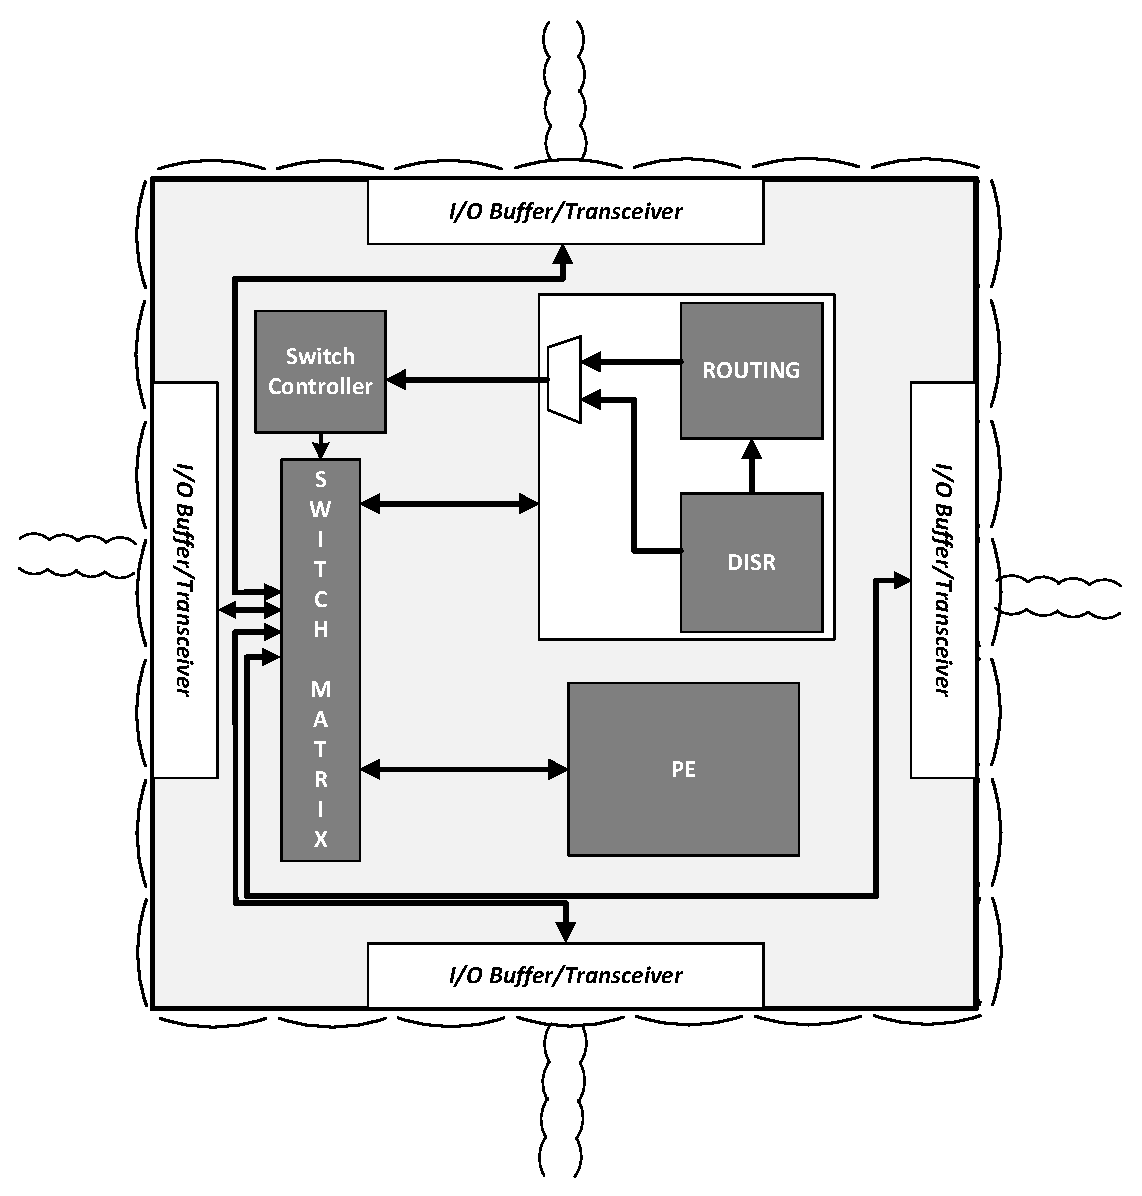
\includegraphics[width=0.45\textwidth]{pictures/node_structure.eps}
  \caption{A possible node structure tailored for a DNA nanonetwork.}
 \label{fig:node_structure}
\end{figure}
%--------------------------------------------------------------------
\subsection{DiSR Architecture}
\label{ssec:disr_architecture}

\begin{figure}
  \centering
  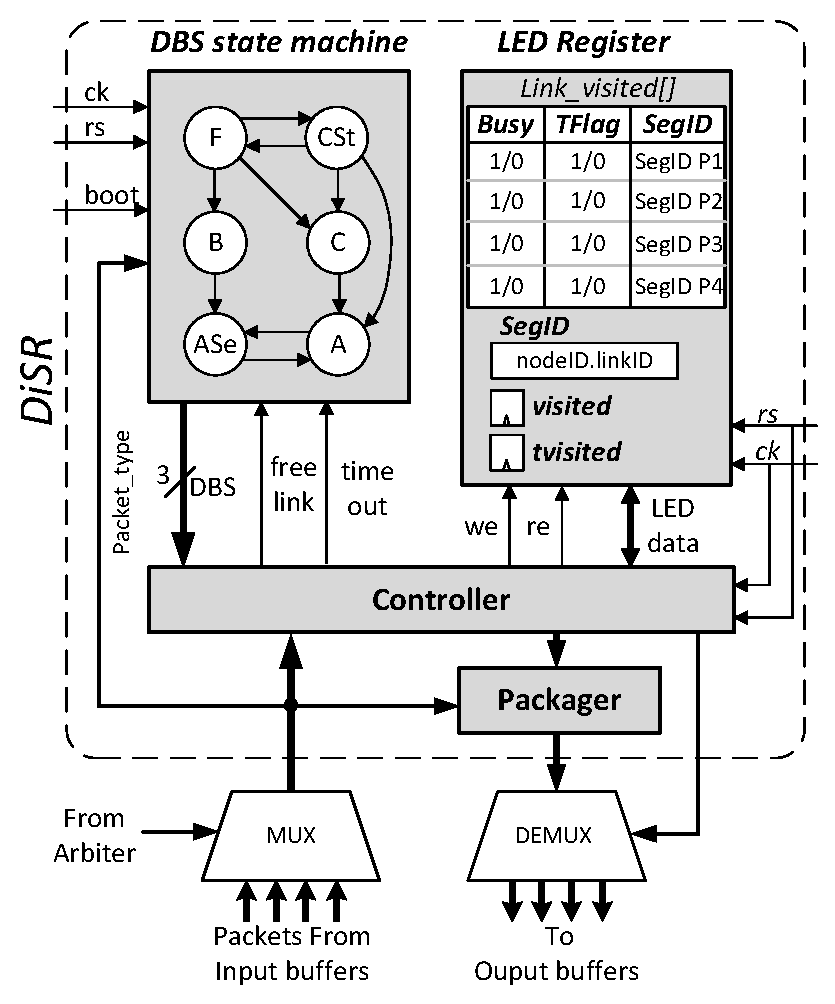
\includegraphics[width=0.40\textwidth]{pictures/disr_rtl_updated.eps}
  \caption{\emph{DiSR} block architecture.}
 \label{fig:implementation}
\end{figure}

To give a basic estimate of the overhead needed we will focus on DiSR-
specific components, that is, the control logic and configuration
registers needed to implement DiSR. In Figure~\ref{fig:implementation}
is shown a sketch of the  architecture, which mainly consist in the
following building elements:

\begin{itemize}

	\item \textbf{DBS block:}

	It takes trace of the DBS state machine,  consisting of a 3-bit
	register (to cover six DBS values) and the  required combinational
	logic. This block receives signals from  stored packets  in order
	to decode the packet type, and from  the control circuitry to
	change its status. The bootstrap node is selected by setting the
	boot signal to high during the initialization phase.

	\item \textbf{LED registers:}
	A set of registers store the \emph{LED} listed in the
	section~\ref{sec:disr_concepts}.  In particular, in the
	link\_visited[] table, can be pointed out the presence of two
	particular registernamed \emph{tflag} and \emph{busy}.  The Latter
	is used to indicate if a specific port is alredy visited or
	tvisited while the former indicates specifically if the specific
	port is alredy candidate or  assigned for a specific segment.

    \item \textbf{Control circuitry:}
    This circuitry decodes the the      incoming packet, the LED
	registers and the DBS,     updating them when required. This block
	drives the LED register   to store or, to read the LED data
	according with \emph{write enable (WE)} or \emph{read enable (RE)}
	signals. Then, the resulting \emph{Ctrl-Out} drives the other
	communication resources for actuating the DiSR routing operation.

	\item \textbf{Packager:}
	Essentially is a set of registers and multiplexers. Starting from
	an incoming packet stored in the input buffer, it updates the
	content of the packet before the retransmission to   a destination
	node.  In some cases, this circuitry builds the packet from the
	scratch.  For example this happens when a node is bootsrap and for
	the first time it should inject a \emph{strating\_segment\_request}. 
	In Fig.~\ref{fig:packager} is shown the architecture of such packager 
	block. When a packet is created for the first time, the multiplexers 
	driven by the controller, will select the information incoming from the 
	internal node such as the \emph{soruce\_ID}. In this situation the 
	TTL field should be resetted to its initial value and the \emph{segment\_ID}
	is composed by the node ID and by the output port identification 
	number.

\end{itemize}

While the elements mentioned above are part of the DiSR circuitry,
the other devices depicted in Fig.~\ref{fig:implementation} like the
multiplexer and demultiplexer are implemented outside DiSR. In
particular, such components will be inside the switch matrix  (refers
to the Fig~\ref{fig:node_structure}).

\begin{figure}
  \centering
  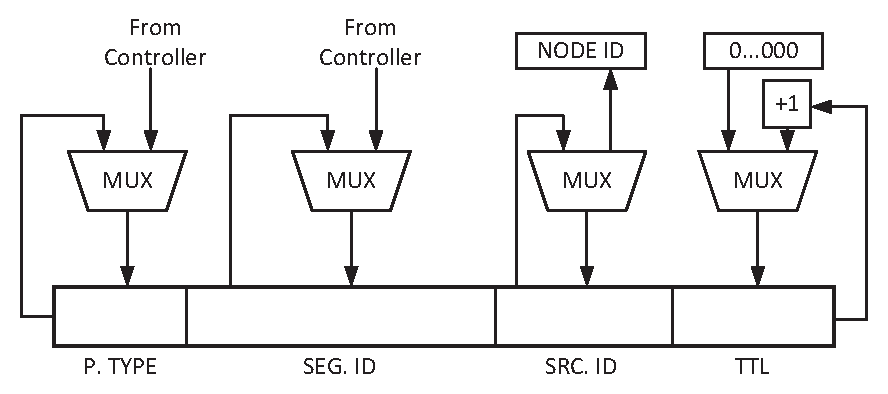
\includegraphics[width=0.40\textwidth]{pictures/packager.eps}
  \caption{Packager block}
 \label{fig:packager}
\end{figure}

\begin{figure}
  \centering
  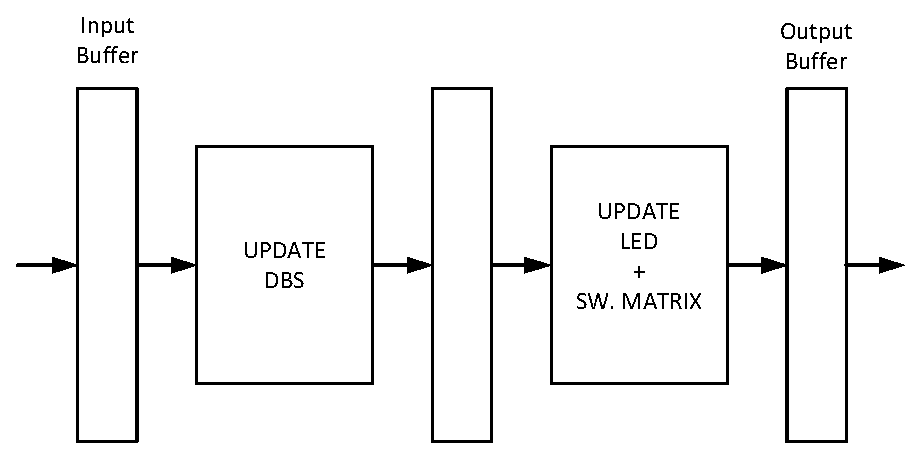
\includegraphics[width=0.40\textwidth]{pictures/pipeline.eps}
  \caption{Pipeline description of DiSR operations}
 \label{fig:pipeline}
\end{figure}

Each of just described building block, reacts with the rising edge  of
the \emph{clock signal}. An asynchronous system \emph{reset} signal is
also present to restore all registers to their default values. When
this signal is set, the DBS state machines for each network
node are set as \emph{Free}.  
In Fig.~\ref{fig:pipeline} is described the pipeline structure of the
DiSR architecture. The packets incoming from the neighbours node, or
locally generated will be send to the DBS state machine in order to te
ensure the status commutation. While the DBS updates its state,  in the
next clock cycle the control circuitry will update the Led status and
will drive the switch matrix in order to send eventually the packets to
the  right output buffer.
%--------------------------------------------------------------------
\subsection{Synthesis results}

As discussed above, one of the main design challenge of DNA Self-
Assembled systems is the limited number of resources available to implement both
computations and routing decisions for each node. Assuming a budget of
$10^4$ CNFETs for each network's node~\cite{liu_jetcs}  we estimated
the required resources to implement the entire DiSR block. The RTL
description of the circuitry described in the last section (with an
hardware description language)  of the DiSR circuitry has been written
and synthesized at gate-level using \emph{Synopsys Design Compiler} with 
a generic technology library (GTECH).
Considering the specific layout of each single logic elements  (NAND,
full-adder, latch etc.), it has been possible to get a rough estimate
of the number of transistors necessary to implement the DiSR logic.
Figure~\ref{fig:synthesys} shows the results of synthesis in terms of
number of devices (CNFETs) versus the number of network nodes while
the network scales up from $10\times10$ to $100\times100$ nodes.

\begin{figure}
  \centering
  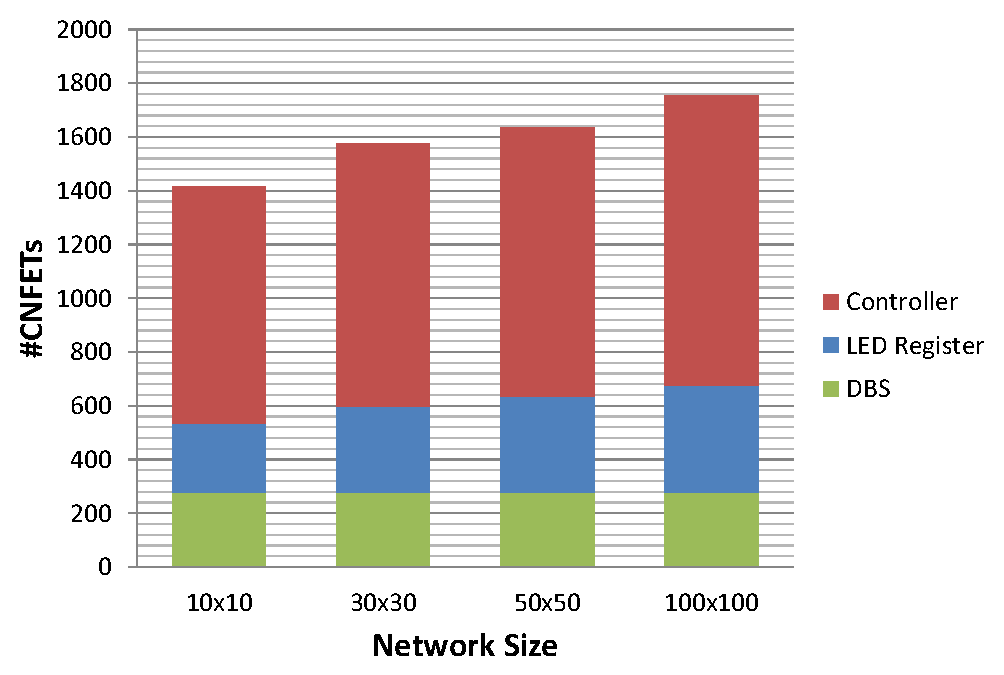
\includegraphics[width=0.50\textwidth]{pictures/synthesis.eps}
  \caption{Number of network's node (N) vs number of CNFETs necassary to implement
  the DiSR circuitry.}
 \label{fig:synthesys}
\end{figure}

In particular, observing the Figure~\ref{fig:synthesys} can  be
pointed out that the proposed implementation occupies about 17,5\% of
the node budget. In particular the main contribution is due to the
controller circuitry followed by LED registers. Further, more than the
absolute number of devices itself, it is interesting to observe that
the circuitry complexity which implements the DiSR algorithm increases
with a slowly growing trend.   An intuitive explanation of this is the
relatively simple logic of DiSR, whose behaviour is almost code on
scalable storage structures. For example, the number of registers
implementing the \emph{link\_visited[]} and \emph{link\_tvisited[]}
table follow the logarithmic function $N_{reg}=N_{port} \cdot
log_2(N)$ where \emph{Nport} is the number of the router’s ports, N is
the number of network’s nodes.

In order to have an idea of the maximum working clock frequency for
the implemented circuitry, timing results can be obtained from a gate-
level netlist. Since a complete technology library usefull for
commercial synthesis tool (like Design Compiler) doesn't exist for 
this particular technology (at the best that we know), we have
synthesized the RTL description of DiSR with a standard 32nm CMOS
library obtaining  a delay of about $\mathrm{\tau_{DiSR}=10} FO4$
(fan-out of four). Considering the results obtained
in~\cite{deng_isscc07}, wich reports the ratio in therms of FO4
between a standard 32nm CMOS technology and a carbon nanotube ones, 
rough delay estimation can be obtained. In particolar has been reported a
ratio R of:  
\begin{equation}
\mathrm{R=\frac{FO4_{CMOS}}{FO4_{CNFET}}=2}  
\end{equation}
Considering that F04 CMOS is about 30 ps, and the results of last
equation, a FO4 for the CNFET case is equal to about 15 ps, and
then the working frequency can be computed as:
\begin{equation}
\mathrm{f_{clk}=\frac{1}{T_{max}}=\frac{1}{\tau_{DiSR} \cdot FO4_{CNFET}}}=
\frac{1}{10\cdot 15 \cdot 10^{-12}}=6,6 GHz
\end{equation}
where $\mathrm{\tau_{DiSR}}$ was expressed in therms of FO4.

Regards the power consumption of the entire DiSR devices, 
an accurate power analysis with the switch activity
annotation can be avoided because the DiSR circuitry will be active 
only once at the system startup. Indeed, after the setup phase, when all segments
are mapped in to the network, the DiSR block will stop its activity
giving as output the fixed status of segments to the routing
algorithm. For this reason the dynamic power will going  to zero and
the only cosumption will be eventually only due to the leackage
consumption.



%------------------------------------------------------------------------------

\section{Conclusions}
In this work we presented DiSR, an initial attempt of porting a segment based
approach to distributed self-assembled nanoscale scenario. We
demonstrated how DiSR can accomplish the aim of finding a segment
coverage of the network without requiring any centralized approach
that would request a graph topology as input. A draft hardware
implementation has been presented to evaluate the impact on the limited
node size typical of the assumed scenario. Future works will focus on
developing self tuning of DiSR to match a high coverage levels and the
detailed low level hardware implementation on
DNA grid using the appropriate nano devices models.

%------------------------------------------------------------------------------

\balance

\bibliographystyle{IEEEtran} 
\bibliography{bibliography}

%------------------------------------------------------------------------------

\end{document}
